\documentclass[11pt,a4paper]{article}
\usepackage[utf8]{inputenc}
\usepackage[margin=1in]{geometry}
\usepackage{amsmath,amssymb}
\usepackage{hyperref}
\usepackage{graphicx}
\usepackage{booktabs}
\usepackage{enumitem}
\usepackage{tikz}
\usetikzlibrary{shapes.geometric, arrows.meta, positioning}

% Hyperlink Setup
\hypersetup{
    colorlinks=true,
    linkcolor=blue,
    citecolor=blue,
    urlcolor=blue
}

\title{\textbf{Project Proposal}\\[0.5em] 
\Large Multi-Scale Integration of Macroscopic fMRI and Mesoscopic Attractor Circuit Models: Decoding Working Memory Modulation of Visual Category Representations}
\author{}
\date{\today}

\begin{document}

\maketitle

\hrule
\vspace{1em}

\section{Motivation \& Background}

A central challenge in cognitive neuroscience is bridging the gap between macroscopic neuroimaging observations and mesoscopic computational mechanisms. While task-based functional Magnetic Resonance Imaging (fMRI) excels at mapping cognitive functions to specific brain networks, the Blood Oxygen Level Dependent (BOLD) signal reflects metabolic energy consumption averaged over millions of neurons and several seconds. Consequently, standard univariate fMRI cannot explain \textit{how} information is dynamically encoded, maintained, and manipulated at the microcircuit level.

In working memory (WM), the classical paradigm assumes that information is maintained through persistent, high-frequency spiking in frontal-parietal circuits. However, persistent spiking is metabolically expensive and susceptible to distraction. Recent biophysical theories, specifically \textbf{Short-Term Synaptic Plasticity (STSP)} based on Tsodyks-Markram dynamics, propose an alternative ``activity-silent'' mechanism. Under STSP, memory items are encoded in transient changes in presynaptic calcium utilization ($u$) and available neurotransmitter resources ($x$), allowing representations to be maintained with minimal spiking during delay intervals.

This project addresses this methodological scale gap by establishing a quantitative, closed-loop pipeline. By integrating \textbf{Human Connectome Project (HCP)} task fMRI (\texttt{tfMRI\_WM}) with \textbf{Representational Similarity Analysis (RSA)}, \textbf{Multivariate Pattern Analysis (MVPA)}, and \textbf{Leaky Integrate-and-Fire (LIF)} attractor network modeling, this project directly connects localized BOLD metabolic demands to specific information content and synaptic calcium dynamics.

\section{Detailed Problem Statement}

Univariate General Linear Model (GLM) analyses consistently demonstrate that high working memory load (e.g., 2-back vs. 0-back) increases BOLD activation across the Frontoparietal/Cingulate control network and modulates activity in visual cortices. However, univariate methods suffer from key theoretical limitations:

\begin{enumerate}
    \item \textbf{Univariate Ambiguity:} Increased BOLD activation in frontoparietal regions could reflect top-down gain control, non-specific attentional recruitment, or the active maintenance of category-specific contents.
    \item \textbf{Representational Geometry under Load:} It remains unresolved whether cognitive load distorts the underlying representational geometry (pairwise dissimilarity) of visual category targets in visual cortices or leaves it structurally invariant.
    \item \textbf{Metabolic-Circuit Gap:} There is no standard framework to prove whether empirical fMRI BOLD parameter estimates ($\beta$) in executive regions match the theoretical metabolic costs of activity-silent STSP maintenance (periodic population refreshes and calcium pump clearance).
\end{enumerate}

\subsection*{Core Research Hypotheses}

\begin{itemize}
    \item \textbf{Hypothesis 1 ($H_1$):} Visual category representations in Occipito-Temporal cortex maintain structural geometric invariance across working memory load states (0-back vs. 2-back).
    \item \textbf{Hypothesis 2 ($H_2$):} Category-specific information emerges dynamically in Frontoparietal/Cingulate control regions under high working memory load (2-back), even if these regions show no category tuning during passive viewing (0-back).
    \item \textbf{Hypothesis 3 ($H_3$):} The theoretical metabolic expenditure (ATP) of periodic population bursts and presynaptic calcium clearance in a simulated STSP circuit quantitatively accounts for the empirical BOLD $\beta$ magnitude observed in task fMRI.
\end{itemize}

\section{Methodology, Simulation Protocol, \& Expected Results}

The project is structured into a sequential three-phase workflow pipeline:

\begin{center}
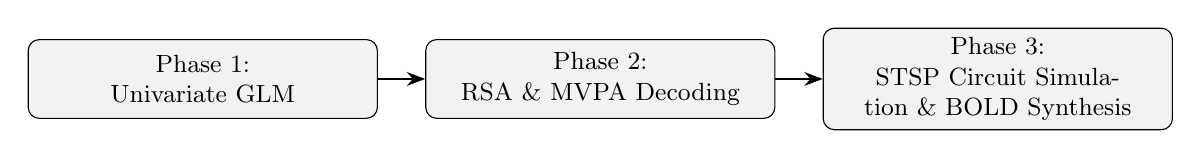
\begin{tikzpicture}[
    node distance=0.6cm, 
    auto, 
    >=Stealth,
    phase/.style={draw, rectangle, rounded corners, align=center, fill=gray!10, text width=4.2cm, font=\small, minimum height=1cm}
]
    \node [phase] (phase1) {Phase 1:\\Univariate GLM};
    \node [phase, right=of phase1] (phase2) {Phase 2:\\RSA \& MVPA Decoding};
    \node [phase, right=of phase2] (phase3) {Phase 3:\\STSP Circuit Simulation \& BOLD Synthesis};
    
    \draw [->, thick] (phase1) -- (phase2);
    \draw [->, thick] (phase2) -- (phase3);
\end{tikzpicture}
\end{center}

\subsection{Phase 1: Signal Extraction \& First-Level GLM Fitting}

\begin{itemize}
    \item \textbf{Data Processing:} Process Left-Right (LR) and Right-Left (RL) phase encoding runs from the HCP \texttt{tfMRI\_WM} task dataset (TR = 0.7s, 2mm isotropic MNI space).
    \item \textbf{Nuisance \& EV Modeling:} Parse 8 experimental Explanatory Variable (EV) conditions:
    \[
    \text{Load } (0\text{-back}, 2\text{-back}) \times \text{Category } (\text{Body}, \text{Face}, \text{Place}, \text{Tool})
    \]
    Extract 6 rigid-body motion parameters (translation and rotation) as nuisance regressors.
    \item \textbf{GLM Contrast Extraction:} Fit a Nilearn \texttt{FirstLevelModel} using a Glover HRF and AR(1) noise model to generate 8 raw effect-size ($\beta$) maps per run relative to implicit fixation.
    \item \textbf{ROI Definition:} Define binary masks for Occipito-Temporal (category-selective visual) and Frontoparietal/Cingulate (load-sensitive control) regions using the Harvard-Oxford probabilistic atlas resampled to the subject BOLD geometry.
\end{itemize}

\subsection{Phase 2: Information Representation (RSA \& Decoding)}

\begin{itemize}
    \item \textbf{Split-Half RSA (Step 4):} Compute cross-run ($LR \leftrightarrow RL$) Pearson dissimilarity matrices ($D = 1 - r$) across the 8 conditions to generate $8 \times 8$ RDMs. Extract $4 \times 4$ category sub-RDMs for 0-back and 2-back conditions.
    \item \textbf{Targeted Gap Test ($H_1$):} Calculate the Spearman rank correlation ($\rho$) between the upper-triangular off-diagonal vectors of the 0-back and 2-back category sub-RDMs to evaluate representational invariance under load.
    \item \textbf{Linear MVPA Decoding (Step 5):} Train Linear Support Vector Machines (SVM) with cross-run fold validation ($LR \leftrightarrow RL$) to perform:
    \begin{enumerate}
        \item 4-way Category Decoding within 0-back and 2-back (Chance = 25\%).
        \item 2-way Binary Load Decoding (0-back vs. 2-back, Chance = 50\%).
        \item Cross-Load Category Generalization (Train on 0-back $\rightarrow$ Test on 2-back) to test $H_2$.
    \end{enumerate}
\end{itemize}

\subsection{Phase 3: Biophysical STSP Circuit Simulation \& BOLD Synthesis}

\begin{itemize}
    \item \textbf{Network Initialization (Step 6):} Construct a biophysical spiking network representing a frontoparietal cortical column containing $N_E = 800$ excitatory pyramidal neurons and $N_I = 200$ inhibitory interneurons. Partition $N_E$ into 4 category-selective pools (100 units/pool) and 1 background pool. Scale intra-pool recurrent gain ($w_+$) using empirical decoding performance from Step 5.
    \item \textbf{Synaptic Dynamics Simulation (Step 7):} Simulate Leaky Integrate-and-Fire (LIF) membrane dynamics alongside Tsodyks-Markram STSP differential equations:
    \begin{align}
        \frac{du}{dt} &= \frac{U_{\text{baseline}} - u}{\tau_F} + U_{\text{baseline}}(1 - u) \sum_k \delta(t - t_k) \\
        \frac{dx}{dt} &= \frac{1 - x}{\tau_D} - u \cdot x \sum_k \delta(t - t_k)
    \end{align}
    Simulate the 2-back maintenance delay (cue presentation $\rightarrow$ activity-silent delay) to model $u$ (calcium utilization) and $x$ (resource availability).
    \item \textbf{LFP \& BOLD Synthesis (Step 8):}
    \begin{enumerate}
        \item Compute Local Field Potentials (LFPs) as aggregate synaptic fluxes and extract Theta (4--8 Hz) and Gamma (30--80 Hz) power spectra using continuous spectrograms.
        \item Calculate total metabolic ATP expenditure ($ATP_{\text{total}}$) combining action potential costs ($C_{\text{AP}}$) and calcium pump clearance costs ($C_{\text{Ca}}$):
        \[
        ATP_{\text{total}}(t) = N_{\text{spikes}}(t) \cdot C_{\text{AP}} + \sum_{i \in E} \max\left(0, \frac{du_i}{dt}\right) \cdot C_{\text{Ca}}
        \]
        \item Convolve $ATP_{\text{total}}(t)$ with a double-gamma Glover HRF to synthesize the predicted BOLD time-series and compare its peak magnitude directly against the empirical First-Level GLM $\beta$ estimate.
    \end{enumerate}
\end{itemize}

\begin{center}
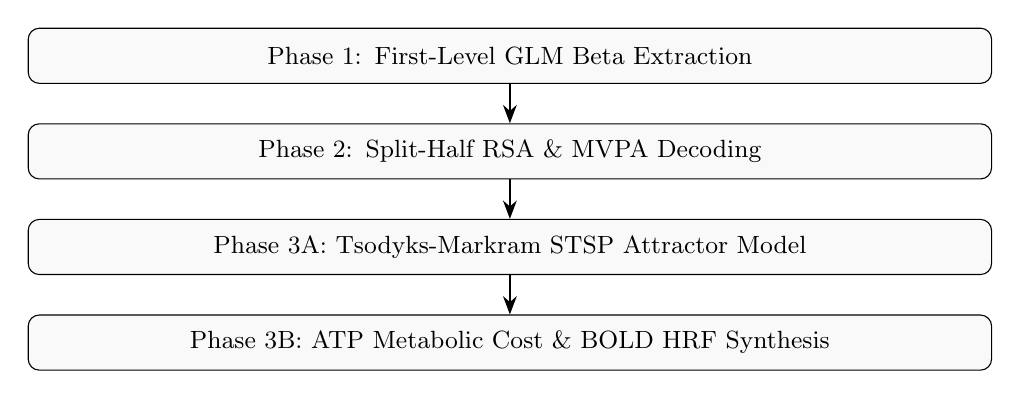
\begin{tikzpicture}[
    node distance=0.5cm, 
    auto, 
    >=Stealth, 
    block/.style={draw, rectangle, rounded corners, align=center, fill=gray!5, text width=12cm, font=\small, minimum height=0.7cm}
]
    \node [block] (step1) {Phase 1: First-Level GLM Beta Extraction};
    \node [block, below=of step1] (step2) {Phase 2: Split-Half RSA \& MVPA Decoding};
    \node [block, below=of step2] (step3) {Phase 3A: Tsodyks-Markram STSP Attractor Model};
    \node [block, below=of step3] (step4) {Phase 3B: ATP Metabolic Cost \& BOLD HRF Synthesis};
    
    \draw [->, thick] (step1) -- (step2);
    \draw [->, thick] (step2) -- (step3);
    \draw [->, thick] (step3) -- (step4);
\end{tikzpicture}
\end{center}

\subsection{Expected Results}

\begin{enumerate}
    \item \textbf{Occipito-Temporal Structural Invariance:} High Spearman rank correlation ($\rho > 0.85, p < 0.001$) between 0-back and 2-back category sub-RDMs in visual cortices, confirming representational invariance under cognitive load ($H_1$).
    \item \textbf{Frontoparietal Dynamic Emergence:} Category decoding accuracy in Frontoparietal cortex rises significantly above chance (25\%) strictly during the 2-back condition, confirming load-dependent recruitment of executive regions for content maintenance ($H_2$).
    \item \textbf{Activity-Silent Memory Trajectory:} Following cue offset, spiking activity in the simulated circuit returns to baseline while synaptic efficacy ($u \cdot x$) remains elevated for $>1500\text{ ms}$, demonstrating silent chemical storage.
    \item \textbf{Model-Data BOLD Alignment:} Synthesized BOLD signals derived from simulated ATP expenditure (spikes + calcium clearance) match empirical GLM $\beta$ magnitudes within a tight ratio ($0.90 - 1.10$), validating the biophysical origin of the fMRI signal ($H_3$).
\end{enumerate}

\section{Novelty, Key References, Code \& Data Repositories}

\subsection{Project Novelty}

\begin{enumerate}
    \item \textbf{Closed-Loop Multi-Scale Bridge:} Unlike standard neuroimaging studies that stop at MVPA decoding, or computational studies that rely on arbitrary network parameters, this project establishes a direct quantitative loop: empirical MVPA performance constrains recurrent attractor gain ($w_+$), and simulated biophysical ATP costs predict empirical fMRI $\beta$ weights.
    \item \textbf{Activity-Silent BOLD Validation:} Provides an explicit metabolic account showing that activity-silent memory traces---maintained via calcium utilization ($u$) and brief refreshing bursts---generate measurable BOLD signals through presynaptic $\text{Ca}^{2+}$ clearance dynamics.
    \item \textbf{Cross-Load Generalization Analysis:} Formally tests the transferability of visual representational codes into executive control networks across differing working memory demands.
\end{enumerate}

\subsection{Key References}

\begin{enumerate}[label={[\arabic*]}]
    \item Tsodyks, M. V., \& Markram, H. (1997). The neural code between neocortical pyramidal neurons depends on neurotransmitter release probability. \textit{Proceedings of the National Academy of Sciences}, 94(2), 719--723.
    \item Mongillo, G., Barak, O., \& Tsodyks, M. (2008). Synaptic theory of working memory. \textit{Science}, 319(5869), 1543--1546.
    \item Stokes, M. G. (2015). ‘Activity-silent’ working memory in prefrontal cortex: a dynamic coding framework. \textit{Trends in Cognitive Sciences}, 19(7), 394--405.
    \item Kriegeskorte, N., Mur, M., \& Bandettini, P. A. (2008). Representational similarity analysis–connecting the branches of systems neuroscience. \textit{Frontiers in Systems Neuroscience}, 2, 4.
    \item Barch, D. M., et al. (2013). Function in the human connectome: Task-fMRI and individual differences in behavior. \textit{NeuroImage}, 80, 169--189.
    \item Haxby, J. V., et al. (2001). Distributed and overlapping representations of faces and objects in ventral temporal cortex. \textit{Science}, 293(5539), 2425--2430.
\end{enumerate}

\subsection{Code \& Data Repositories}

\begin{itemize}
    \item \textbf{Primary Dataset:} Human Connectome Project (HCP) Young Adult 1200 Subjects Release (\texttt{tfMRI\_WM} Working Memory Task Dataset, volume-space preprocessed NIfTI files and 3-column EV text files).
    \item \textbf{Software Stack \& Libraries:}
    \begin{itemize}
        \item \texttt{Python 3.8+}
        \item \texttt{Nilearn} (First-Level GLM modeling, atlas management, NiftiMasker pattern extraction)
        \item \texttt{NiBabel} (Neuroimaging NIfTI image manipulation)
        \item \texttt{Scikit-Learn} (Linear Support Vector Machines, StandardScaler, cross-validation pipelines)
        \item \texttt{SciPy} (Spearman rank correlation, spectrogram signal analysis, gamma distribution functions)
        \item \texttt{Pandas} / \texttt{NumPy} (EV table parsing, vector operations, Euler integration)
        \item \texttt{Matplotlib} / \texttt{Seaborn} (RDM heatmaps, raster plots, spectral and BOLD time-series visualization)
    \end{itemize}
    \item \textbf{Pipeline Code Repository Structure:}
    \begin{itemize}
        \item \texttt{Phase1\_GLM\_Condition\_Mapping.py}: EV parsing, motion regression, and Nilearn FirstLevelModel fitting.
        \item \texttt{Phase1\_ROI\_Pattern\_Extraction.py}: Harvard-Oxford atlas masking and voxel pattern vector extraction.
        \item \texttt{Phase2\_Split\_Half\_RSA.py}: $8 \times 8$ cross-run RDM construction and rank correlation testing.
        \item \texttt{Phase2\_MVPA\_Decoding.py}: 4-way category, 2-way load, and cross-load linear SVM decoding.
        \item \texttt{Phase3\_STSP\_Network\_Init.py}: Biophysical neuron pool setup and connectivity matrix ($W$) initialization.
        \item \texttt{Phase3\_STSP\_Synaptic\_Simulation.py}: LIF Euler integration and Tsodyks-Markram $u, x$ differential equation solver.
        \item \texttt{Phase3\_Synthesis\_BOLD\_Prediction.py}: LFP spectrogram generation, ATP metabolic cost calculation, and Glover HRF BOLD synthesis.
    \end{itemize}
\end{itemize}

\end{document}